% ---------------------------------------------------------------
% Preamble
% ---------------------------------------------------------------
%\documentclass[a4paper,fleqn,longmktitle]{cas-sc}
\documentclass[a4paper,fleqn]{cas-dc}
%\documentclass[a4paper]{cas-dc}
%\documentclass[a4paper]{cas-sc}
% ---------------------------------------------------------------
% Make margins bigger to fit annotations. Use 1, 2 and 3. TO be removed later
%\paperwidth=\dimexpr \paperwidth + 6cm\relax
%\oddsidemargin=\dimexpr\oddsidemargin + 3cm\relax
%\evensidemargin=\dimexpr\evensidemargin + 3cm\relax
%\marginparwidth=\dimexpr \marginparwidth + 3cm\relax
% -------------------------------------------------------------------- 
% Packages
% --------------------------------------------------------------------
% Figure packages
\usepackage{graphicx,float}
\usepackage{adjustbox}
% Text, input, formatting, and language-related packages
\usepackage[T1]{fontenc}
\usepackage{subcaption}

\usepackage{csvsimple}

% TODO package
\usepackage[bordercolor=gray!20,backgroundcolor=blue!10,linecolor=black,textsize=footnotesize,textwidth=1in]{todonotes}
\setlength{\marginparwidth}{1in}
% \usepackage[utf8]{inputenc}
% \usepackage[nomath]{lmodern}

% Margin and formatting specifications
%\usepackage[authoryear]{natbib}
\usepackage[sort]{natbib}
\setcitestyle{square,numbers}

 %\bibliographystyle{cas-model2-names}

\usepackage{setspace}
\usepackage{subfiles} % Best loaded last in the preamble

% \usepackage[authoryear,longnamesfirst]{natbib}

% Math packages
\usepackage{amsmath, amsthm, amssymb, amsfonts, bm, nccmath, mathdots, mathtools, bigints, ulem}

\usepackage{tikz}
\usepackage{pgfplots}
\usetikzlibrary{shapes.geometric,angles,quotes,calc}

\usepackage{placeins}

\usepackage[final]{pdfpages}

% --------------------------------------------------------------------
% Packages Configurations
\usepackage{enumitem}
% --------------------------------------------------------------------
% (General) General configurations and fixes
\AtBeginDocument{\setlength{\FullWidth}{\textwidth}}	% Solves els-cas caption positioning issue
\setlength{\parindent}{20pt}
%\doublespacing
% --------------------------------------------------------------------
% Other Definitions
% --------------------------------------------------------------------
\graphicspath{{Figures/}}
% --------------------------------------------------------------------
% Environments
% --------------------------------------------------------------------
% ...

% --------------------------------------------------------------------
% Commands
% --------------------------------------------------------------------

% ==============================================================
% ========================== DOCUMENT ==========================
% ==============================================================
\begin{document} 
%  --------------------------------------------------------------------

% ===================================================
% METADATA
% ===================================================
\title[mode=title]{Parameter estimation}                      
\shorttitle{Parameter estimation}

\shortauthors{OS, PO}

\author[1]{Oliwer Sliczniuk}[orcid=0000-0003-2593-5956]
\ead{oliwer.sliczniuk@aalto.fi}
\cormark[1]
\credit{a}

\author[1]{Pekka Oinas}[orcid=0000-0002-0183-5558]
\credit{b}

%\author[1]{Francesco Corona}[orcid=0000-0002-3615-1359]
%\credit{c}

\address[1]{Aalto University, School of Chemical Engineering, Espoo, 02150, Finland}
%\address[2]{2}

\cortext[cor1]{Corresponding author}

% ===================================================
% ABSTRACT
% ===================================================
\begin{abstract}
%Given a system of partial differential equations, $F(t,x,\dot{x},p,u)=0$, where $x$ represents state variables, $p$ is the parameters, and $u$ are control variables, the process model is simultaneously solved for both $x_i$ and a set of sensitivity functions, $dx_i/dp_j$, overall times $t$.These sensitivity functions measure the influence of the parameter change on the model's output. As an example, the supercritical extraction process is presented. The impact of mass flow rate, pressure, and inlet temperature on the model's output is discussed. The sensitivity analysis results prove that the considered variables can affect the extraction's yield and be used as control variables in optimization problems. Moreover, the local sensitivity analysis results are analyzed from a phenomenological point of view to enhance understanding of the process model.
%Given a system of partial differential equations, $F(t,x,\dot{x},\Theta,u)=0$, where $x$ represents state variables, $\Theta$ are the parameters, and $u$ are control variables, we describe the supercritical extraction process. The process model describes a partially filled extractor with a fixed bed, which work under constant operating conditions. We assume that the flow is uniform across any cross-section, although the area available for the fluid phase can change along the extractor. We apply the concept of quasi-one-dimensional flow to mimic the modelling of a two-dimensional case.
%In this work, a distributed-parameter model, based on \citet{Reverchon1996} is used to describe a fluid-solid extraction process of caraway oil from caraway seeds with $CO_2$ as a solvent. The model parameters such as partition factor, internal diffusion coefficient, axial diffusion coefficient \textit{and saturation concentration} are obtained from parameter estimation. The parameters are estimated based on four experiments performed at $40^\circ C$/$200$ bar, $50^\circ C$/$200$ bar, $40^\circ C$/$300$ bar and $50^\circ C$/$300$ bar. Given yield data, the model-based parameter estimation uses the maximum likelihood estimation method under assumption of normal error.
This study aimed to investigate the supercritical extraction process of the caraway oil from caraway seeds. The extraction was performed in a partially filled extractor with a fixed bed operated under multiple constant operating conditions. The dataset collected from four experiments consists of four experiments conducted at different operating conditions: $40~^\circ C$ / $200$ bar, $50~^\circ C$ / $200$ bar, $40~^\circ C$ / $300$ bar, and $50~^\circ C$ / $300$ bar. A distributed-parameter model is used to describe the fluid-solid extraction process with carbon dioxide as a solvent. The concept of quasi-one-dimensional flow is applied to reduce the number of spatial dimensions. The flow is assumed to be uniform across any cross-section, although the area available for the fluid phase can vary along the extractor. This model requires parameters such as partition factor, internal diffusion coefficient, axial diffusion coefficient, saturation concentration, and an initial state estimate. These parameters are estimated from the Peng-Robinson equation of state and by applying the maximum likelihood estimation method on yield data under the normal error assumption. 

\end{abstract}

\begin{keywords}
Supercritical extraction \sep Parameter estimation \sep Mathematical modelling
\end{keywords}

% ===================================================
% TITLE
% ===================================================
\maketitle

% ===================================================
% Section: Introduction
% ===================================================\section{Introduction}

\section{Introduction}
%\subfile{Sections/introduction}
\subfile{Sections/introduction_imp}

\section{Materials and methods} \label{CH: Materials and methods}

\subsection{Supercritical fluids} \label{CH: Thermodynamic}
%\subfile{Sections/Thermo}
\subfile{Sections/Thermo_imp}

%\clearpage
%\subfile{Sections/Materials_and_methods}

\subsection{Governing equations} \label{CH:Governing_equations_chapter}
%\footnote{For the sake of clarity of the process model, different colors have been used in the equations to indicate: 
%	{\color{red}control variables},
%	{\color{black}state variables},
%	{\color{black}variables} and
%	{\color{black}parameters}.} 
	The governing equation for a quasi-one-dimensional compressible flow in Cartesian coordinates can be found in the Appendix \ref{CH: Gouverning equations} and in the work of \citet{Anderson1995}. Quasi-one-dimensional flow is a fluid flow characterized by the assumption that the flow properties remain uniform across any given cross-section of the flow. This assumption is made when there is a variation in the cross-sectional area of the flow channel, such as an irregular shape or partial filling of an extractor. In such cases, the flow is considered to be quasi-one-dimensional because the velocity and other flow properties are assumed to vary only in the direction of flow.

The quasi-one-dimensional compressible Navier-Stokes equations in Cartesian coordinates are given by Equations \ref{EQ: CompressibleEuler_1} to \ref{EQ: CompressibleEuler_3}. The derivation of these Equations are presented in Appendix \ref{CH: Gouverning equations}.

{\footnotesize
	\begin{align}
		\label{EQ: CompressibleEuler_1}
		\cfrac{\partial \left( {\color{black}\rho_f} {\color{black}A_f}(z) \right) }{\partial t} + \cfrac{\partial \left( {\color{black}\rho_f} {\color{black}A_f}(z) v \right)}{\partial z} &= 0 \\
		\cfrac{\partial \left( {\color{black}\rho_f} v {\color{black}A_f}(z) \right) }{\partial t} + \cfrac{\partial \left( {\color{black}\rho_f} {\color{black}A_f}(z) v^2 \right)}{\partial z} &= -{\color{black}A_f}(z) \cfrac{\partial {\color{black}P}}{\partial z} \label{EQ: CompressibleEuler_2} \\
		\cfrac{\partial \left( {\color{black}\rho_f} {\color{black}e} {\color{black}A_f}(z) \right) }{\partial t} + \cfrac{\partial \left( {\color{black}\rho_f} {\color{black}A_f}(z) v {\color{black}e}\right)}{\partial z} &= -{\color{black}P}\cfrac{\left( {\color{black}A_f}(z) v \right)}{\partial z} + \cfrac{\partial}{\partial z} \left( \cfrac{\partial {\color{black}T}}{\partial z} \right)   
		\label{EQ: CompressibleEuler_3}
	\end{align}  
}

where ${\color{black}\rho_f}$ is the density of the fluid, ${\color{black}A_f}(z)$ is the function which describe change of the cross-section, $v$ is the velocity, ${\color{black}P}$ is the total pressure, ${\color{black}e}$ is the internal energy of the fluid, $t$ is time and $z$ is the spacial direction.

Based on governing equations, the small discontinuity (defined as $\delta$) in flow properties, shown in Figure \ref{fig: Discontinuity_slow_flow}, can be analysed. The analysis follows the work of \citet{Schreier1982}.

\begin{figure}[!h]
	\centering
	\resizebox{0.95\columnwidth}{!}{%
		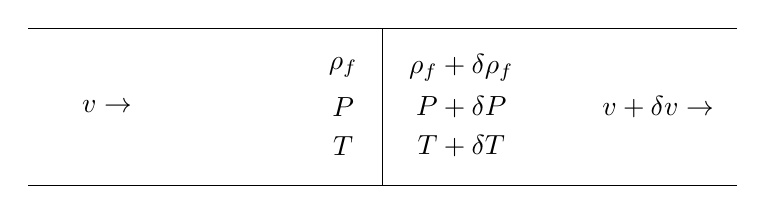
\begin{tikzpicture}[]
			\draw (0,2) -- (9,2);	% Top line
			\draw (0,0) -- (9,0); 	% Bottom line
			\draw (4.5,0) -- (4.5,2); 	% Bottom line
			\node at (4,1.5) {${\color{black}\rho_f}$};
			\node at (5.5,1.5) {${\color{black}\rho_f}+\delta{\color{black}\rho_f}$};
			\node at (4,1.0) {${\color{black}P}$};
			\node at (5.5,1.0) {${\color{black}P}+\delta {\color{black}P}$};
			\node at (4,0.5) {${\color{black}T}$};
			\node at (5.5,0.5) {${\color{black}T}+\delta {\color{black}T}$};
			\node at (1,1.0) {$v \rightarrow$};
			\node at (8,1.0) {$v + \delta v \rightarrow$};
	\end{tikzpicture} }
	\caption{Small discontinuity in one-dimensional flow}
	\label{fig: Discontinuity_slow_flow}
\end{figure} 

The discontinuity is presumed to be at rest relative, and the balance equations become		

{\footnotesize
	\begin{align*}
		&{\color{black}\rho_f} \delta v + v \delta {\color{black}\rho_f} + \delta {\color{black}\rho_f} \delta v = 0 \\
		&\delta {\color{black}P} = \delta v \delta {\color{black}\rho_f}
	\end{align*}
}

These relations are equally valid if the two regions are separated by a region of finite width rather than a discontinuity. 

{\footnotesize
	\begin{equation*}
		\lim_{{\color{black}\rho_f} v \rightarrow 0} {\color{black}\rho_f} \delta v + v \delta {\color{black}\rho_f} + \delta {\color{black}\rho_f} \delta v = 0 / \delta {\color{black}\rho_f} \rightarrow \cfrac{d v}{d {\color{black}\rho_f}} = - \cfrac{v}{{\color{black}\rho_f}}
	\end{equation*}
}

By combining the momentum equation with the above equation, we get

{\footnotesize
	\begin{equation} \label{EQ: Pressure_Velocity}
		\cfrac{d v}{d {\color{black}\rho_f}} = - \cfrac{d v}{d{\color{black}P}} \cfrac{d {\color{black}P}}{d {\color{black}\rho_f}} = -\cfrac{1}{\rho v} \cfrac{d{\color{black}P}}{d{\color{black}\rho_f}} = -\cfrac{v}{{\color{black}\rho_f}}
	\end{equation}
}

Suppose the flow is presumed to be isentropic, $d{\color{black}P}/d{\color{black}\rho_f} = c^2$, so $v^2=c^2$, where $c$ is the speed of sound. This can be interpreted as a small pressure wave propagating with the speed of sound relative to the flow. Moreover, if the flow velocity is relatively low, all pressure changes are hydrodynamic (due to velocity motion) rather than thermodynamic which leads to $\partial {\color{black}\rho_f} / \partial {\color{black}P} \approx 0$. In other words, the small changes in pressure due to flow velocity changes do not change the density. %This has a secondary effect -- the speed of sound in the fluid is $\partial {\color{black}P}/\partial {\color{black}\rho_f} = \infty$ in this instance. So there is an infinite speed of sound, which makes the equations elliptic in nature. It can be deduced that at the isothermal conditions, the density in the system propagates with the same speed as pressure since they are both connected through the equation of state. The details of the Mach-number analysis are presented in Appendix \ref{CH:Low_Mach_chapter}.

\subsection{Extraction model} \label{CH: Extraction_model}
\subfile{Sections/Model}

%\newpage
%\section{Bayes theorem} \label{CH: Bayes}
%\subfile{Sections/Bayes_Theorem}
%\clearpage

\subsection{Parameter estimation} \label{CH: Parameter_estimation}
\subfile{Sections/Parameter_estimation}

\subsection{Experimental work}
\subfile{Sections/Experiments}

\section{Results}
\subfile{Sections/Results}

\section{Conclusions} \label{CH: Conclusion}

This study presented basic aspects regarding the laboratory work for obtaining caraway extracts using supercritical carbon dioxide at different operating conditions. A first-principle process model was developed based on governing equations. Based on the literature review, the extraction kinetic model was selected and combined with the general mass balance equations. The values of unknown parameters in the process model were obtained by parameter estimation. The yield data from the experiments were compared against the yield data generated by the model. The IPOPT solver was used to solve the maximum likelihood estimation. The process model was found to have good agreement with experimental yield curves. Later, the parameters found for each experiment were combined to obtain more general relationships. The correlations for diffusion and decay coefficients are presented as a function of fluid density or Reynolds number. It should be noted that obtained correlations have been prepared with a limited amount of data. These correlations can be used to study qualitatively the impact of different operating conditions on the extraction yield by different methods, such as sensitivity analysis. Moreover, the generalized model could be useful in finding the optimal operating conditions with respect to the process economy.

% ===================================================
% Bibliography
% ===================================================
%% Loading bibliography style file
\clearpage
%\bibliographystyle{model1-num-names}
\bibliographystyle{unsrtnat}
\bibliography{mybibfile}

\clearpage \appendix \label{appendix}
\section{Appendix} 
\subsection{Thermodynamic}
\subfile{Sections/Thermodynamic_details}

\subsection{Governing equations}
\subfile{Sections/Gouverning_equation_derivation}

%\subsection{Low Mach number expansion} \label{CH:Low_Mach_chapter}
%\subfile{Sections/Low_mach_number_expansion}
%\subfile{Sections/Low_mach_number_expansion_imp}

\subsection{Cardano's Formula} \label{CH: Cardano}
\subfile{Sections/Cardano}

\subsection{Initial and boundary conditions} \label{CH: IC_BC}
\subfile{Sections/IC_BC}

%\subsection{Bayes theorem} \label{CH: Bayes}
%\subfile{Sections/Bayes_Theorem}

\subsection{Maximum likelihood} \label{CH: ML}
\subfile{Sections/Likelihood}

\subsection{Solid density measurement} \label{CH: Solid_Density_Measurment}

Figure \ref{fig:density_cal} shows results of density measurement performed with pycnometer.

\begin{figure}[!h]
	\centering 
	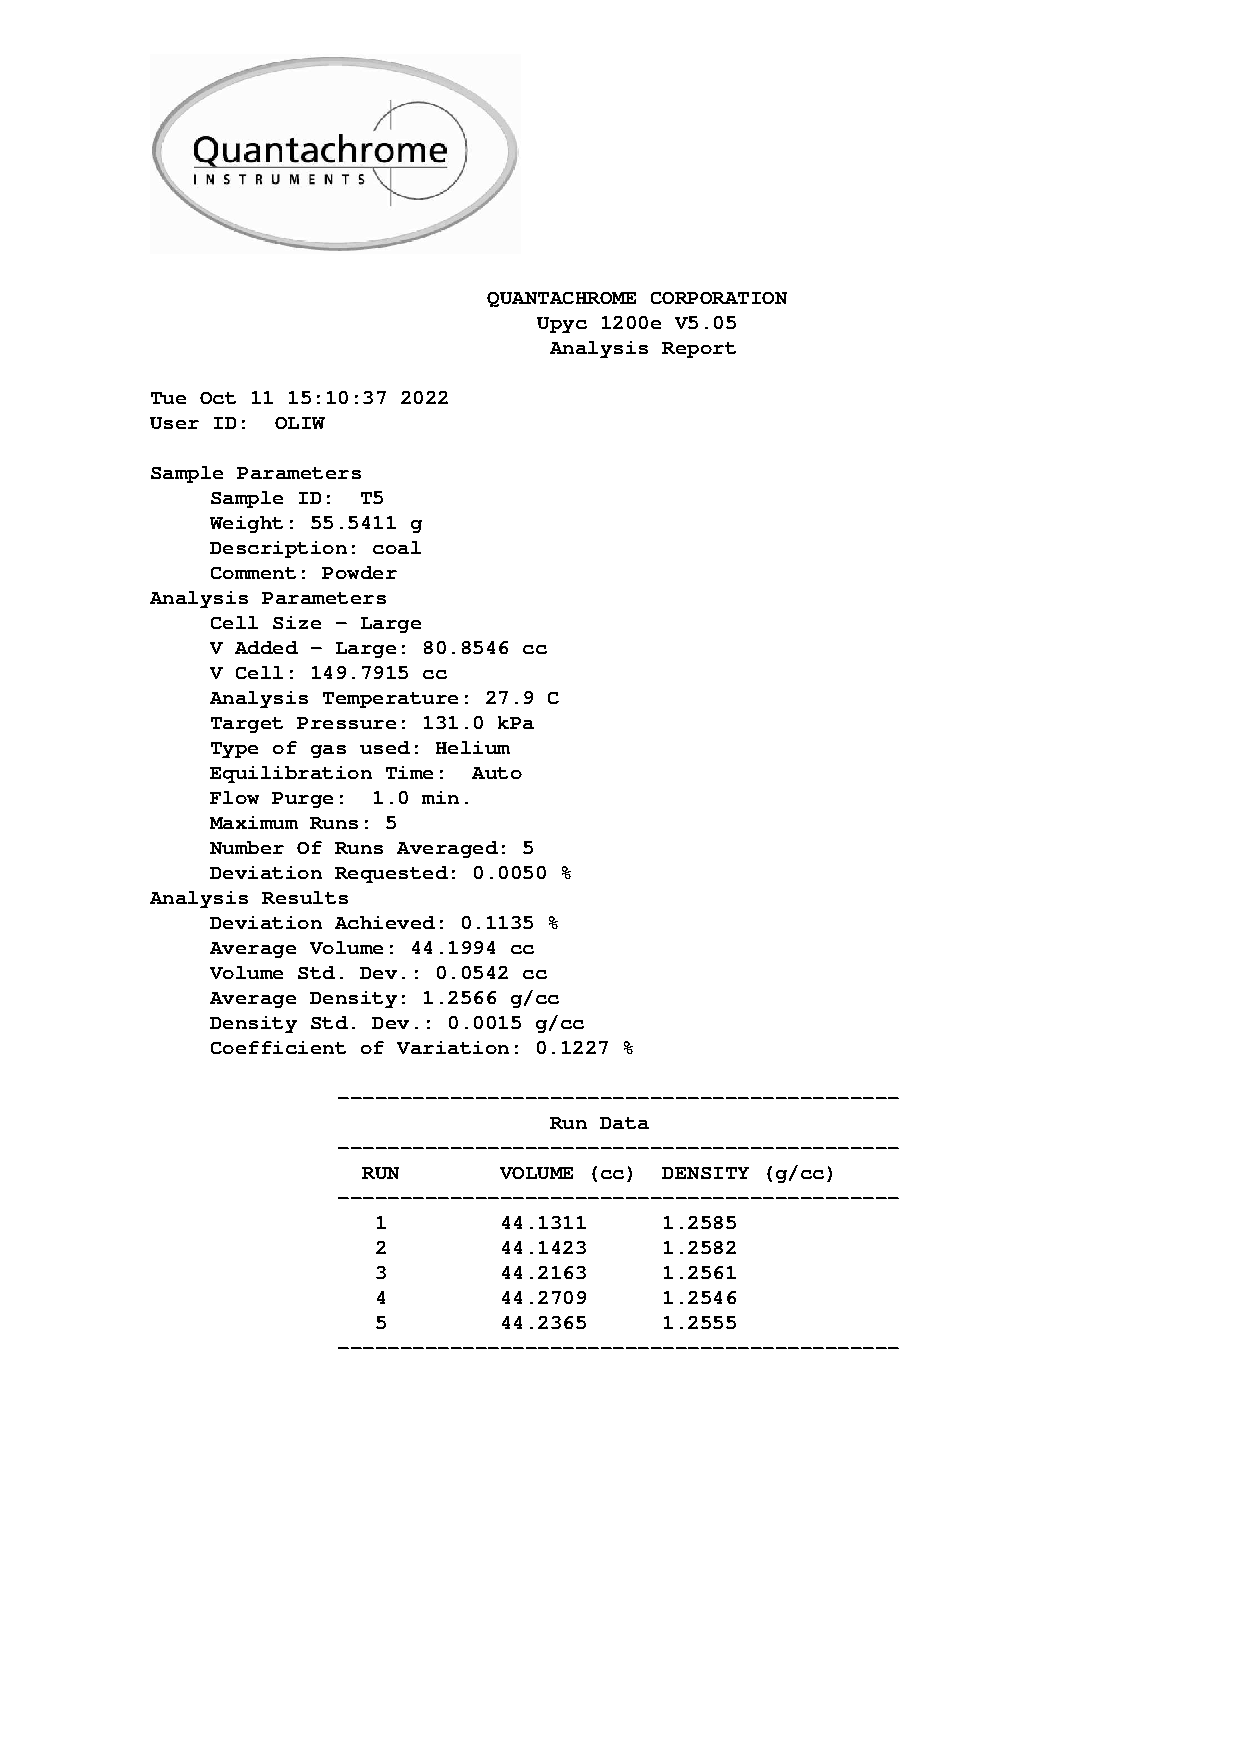
\includegraphics[trim=2cm 6cm 4cm 0cm, clip,width=\columnwidth]{Sections/ultraReportT5.pdf}
	\caption{The result of solid density measurement}
	\label{fig:density_cal}
\end{figure}

{\footnotesize
	\begin{equation*}
		\rho_s^{ave} = \frac{1.2585+1.2582+1.2561+1.2546+1.2555}{5} = 1.25658 [g/cc]
	\end{equation*}
}

\subsection{Porosity calculations} \label{CH: Porosity}
\subfile{Sections/Porosity}

%\subsection{Concentration profiles} \label{CH: Profiles}
%\subfile{Sections/Profiles}

%\subsection{Solution of the parameter estimation starting from another initial guess} \label{CH: Profiles_2}
%\subfile{Sections/Parameter_estimation_solution_from_another_IG}

\iffalse
\newpage
\begin{table*}[p]
		\caption{Notation}
		\label{tab::symbols}
		\begin{tabular}{ |c|l|c| } 
			\hline
			Symbol 		& 	Description 							& Unit 						\\ \hline
			$A$			&	cross-section							& $m^2$ 					\\ \hline
			$c$			&	concentration in fluid phase			& $kg ~ m^{-3}$				\\ \hline
			$Cp$		&	specific heat of the fluid				& $J ~ mol^{-1} ~ K^{-1}$ 	\\ \hline
			$Cp_s$		&	specific heat of the solid				& $J ~ mol^{-1} ~ K^{-1}$ 	\\ \hline
			$D_e^M$		&	axial mass diffusion coefficient		& $m^2 ~ s^{-1}$			\\ \hline
			$D_e^T$		&	axial heat diffusion coefficient		& $m^2 ~ s^{-1}$			\\ \hline
			$Di$		&	internal diffusion coefficient			& $m^2 ~ s^{-1}$			\\ \hline
			$dp$		&	particle diameter						& $m$						\\ \hline
			$F(t)$		&	mass flow-rate							& $kg ~ s^{-1}$				\\ \hline
			$km$		&	partition coefficient					& $[-]$						\\ \hline
			$k^T$		&	thermal conductivity					& $W ~ m^{-1} ~ K^{-1}$		\\ \hline
			$l$			&	characteristic dimension				& $m$						\\ \hline
			$L$			&	total length of the bed					& $m$						\\ \hline
			$m$			&	mass of the oil in solid phase			& $kg$						\\ \hline
			$m_0$		&	initial mass of the oil in solid phase	& $kg$						\\ \hline
			$M_{CO_2}$	&	molecular mass of CO2					& $mol ~ kg^{-1}$			\\ \hline
			$Np$		&	number of model parameters and control variables & $[-]$			\\ \hline
			$N_{\theta}$&	number of model parameters				& $[-]$						\\ \hline
			$Nu$		&	number of control variables				& $[-]$						\\ \hline
			$Nz$		&	number of grid points in z-direction	& $[-]$						\\ \hline
			$p$			&	vector of model parameters and control variables	& $[-]$			\\ \hline
			$P(t)$		&	pressure								& $bar$						\\ \hline
			$Pe$		&	Peclet's number							& $[-]$						\\ \hline
			$q$			&	concentration in solid phase			& $kg ~ m^{-3}$				\\ \hline
			$R$			&	gas constant							& $J ~ K^{-1} ~ mol^{-1}$	\\ \hline
			$Re$		&	Reynolds number							& $[-]$						\\ \hline
			$t$			&	time									& $s$						\\ \hline
			$T$			&	temperature								& $K$						\\ \hline
			$T_0$		&	initial temperature						& $K$						\\ \hline
			$V$			&	volume of the extractor					& $m^3$						\\ \hline
			$y$			&	yield	 								& $[-]$						\\ \hline
			$z$			&	length									& $m$						\\ \hline
			$Z$			&	compressibility	factor					& $[-]$						\\ \hline
			$\epsilon$	&	void fraction							& $[-]$						\\ \hline
			$\rho$		&	density of the fluid					& $kg ~ m^{-3}$				\\ \hline
			$\rho_s$	&	solid density							& $kg ~ m^{-3}$				\\ \hline
			$\mu$		&	shape coefficient						& $[-]$						\\ \hline
			$\theta$	&	vector of model parameters				& $[-]$						\\ \hline
			$\eta$		&	viscosity								& $cP$						\\ \hline				
						& 											&							\\ \hline			
		 	Subscript	& 											&							\\ \hline
			$0$			&	initial conditions						& $[-]$						\\ \hline
			$^*$		&	equilibrium conditions					& $[-]$						\\ \hline							
		\end{tabular}
\end{table*}
\fi
\end{document}